\documentclass[a4paper,12pt]{report}
\usepackage{color}
\usepackage{hyperref}
\hypersetup{
    colorlinks,
    citecolor=black,
    filecolor=black,
    linkcolor=black,
    urlcolor=black
}
\setcounter{secnumdepth}{0}
\usepackage{graphicx}
\usepackage{epstopdf}
\usepackage{amsmath}
\usepackage[table,xcdraw]{xcolor}
\usepackage{amssymb}
\usepackage{listings}
\definecolor{anti-flashwhite}{rgb}{0.95, 0.95, 0.96}
\lstset{
	language=C++,
    basicstyle=\ttfamily,
    keywordstyle=\color{blue}\ttfamily,
    stringstyle=\color{red}\ttfamily,
	commentstyle=\color{green}\ttfamily,
    morecomment=[l][\color{magenta}]{\#},
    backgroundcolor=\color{anti-flashwhite}
}
\begin{document}
\title{
\textbf{Operating Systems - II: CS3523}\\~\\
\begin{large}
\textbf{Programming Assignment - III\\~\\Solving Producer Consumer Problem\\using Semaphores
\& Locks\\}
\end{large}
\begin{large}
\textbf{Assignment Report}
\end{large}
}
\author{\textbf{Sagar Jain - CS17BTECH11034}\\}
\maketitle
\begin{large}
\tableofcontents
\end{large}
\newpage
\section{Salient Features of Program Design}
The problem has been solved using semaphores and locks.
\subsection{Semaphores}
Semaphores have been implemented using the header \textbf{\textit{semaphore.h}}
\begin{enumerate}
\item I have used three semaphores, \textbf{\textit{full}}, \textbf{\textit{empty}} and \textbf{\textit{locker}}.
\item \textbf{\textit{locker}} is initialised as 1, \textbf{\textit{full}} as 0 and \textbf{\textit{empty}} as the capacity of the buffer.
\item \textbf{\textit{full}} is used in the consumer thread to ensure that no consumer can consume if there are no full buffers and we increment it in the producer thread everytime something is produced.
\item \textbf{\textit{empty}} is used in the producer thread to ensure that no producer can produce if there are no empty buffers and we decrement it in the consumer thread everytime something is consumed.
\item \textbf{\textit{locker}} is used to ensure mutual exclusion between multiple producers and consumers.
\item \textbf{Algorithm}\\\\
\textbf{For Producer}:
\begin{lstlisting}
sem_wait(&empty);
sem_wait(&locker);
// produce item
sem_post(&locker);
sem_post(&full);
\end{lstlisting}
\textbf{For Consumer}:
\begin{lstlisting}
sem_wait(&full);
sem_wait(&locker);
// consume item
sem_post(&locker);
sem_post(&empty);
\end{lstlisting}
\end{enumerate}
\subsection{Locks}
Mutex has been implemented using the header \textit{\textbf{mutex}}.
\begin{enumerate}
\item I have used one lock \textbf{\textit{check\_lock}}. \textbf{\textit{counter}} is used to keep the count of the number of filled buffer cells.
\item \textbf{\textit{check\_lock}} is used to ensure that no two processes read the same value of counter and update them leading to a race condition.
\item \textbf{\textit{check\_lock}} also makes sure that production and consumption does not overlap.
\item \textbf{Algorithm}\\\\
\textbf{For consumer}:
\begin{lstlisting}
while(true) {
	check_lock.lock();
	if(counter > 0) {
		counter --;
		break;
	}
	check_lock.unlock();
}
// consume item
check_lock.unlock();
\end{lstlisting}
Similarly, for \textbf{producer}. (counter $<$ capacity)
\begin{lstlisting}
while(true) {
	check_lock.lock();
	if(counter < capacity) {
		counter ++;
		break;
	} 
	check_lock.unlock();
}
// produce item
check_lock.unlock();
\end{lstlisting}
\end{enumerate}
\newpage
\section{Program Output}
The programs output log files (\textit{output-semaphore.txt}, \textit{output-lock.txt}). These files have the data about the point in time at which any consumer or producr consumes or produces any item from or into the buffer.
For Example:\\\\
\textit{14th item produced by thread 4 at 19:58:09 into buffer location 61\\
0th item read from the buffer by thread 0 at 19:58:09 from buffer location 60\\
1th item read from the buffer by thread 0 at 19:58:11 from buffer location 59}
\newpage
\section{Results \& Graphs}
\begin{center}
\begin{large}
\textbf{Producer Waiting Times vs Ratio of Mean Waiting Times}\\
\end{large}
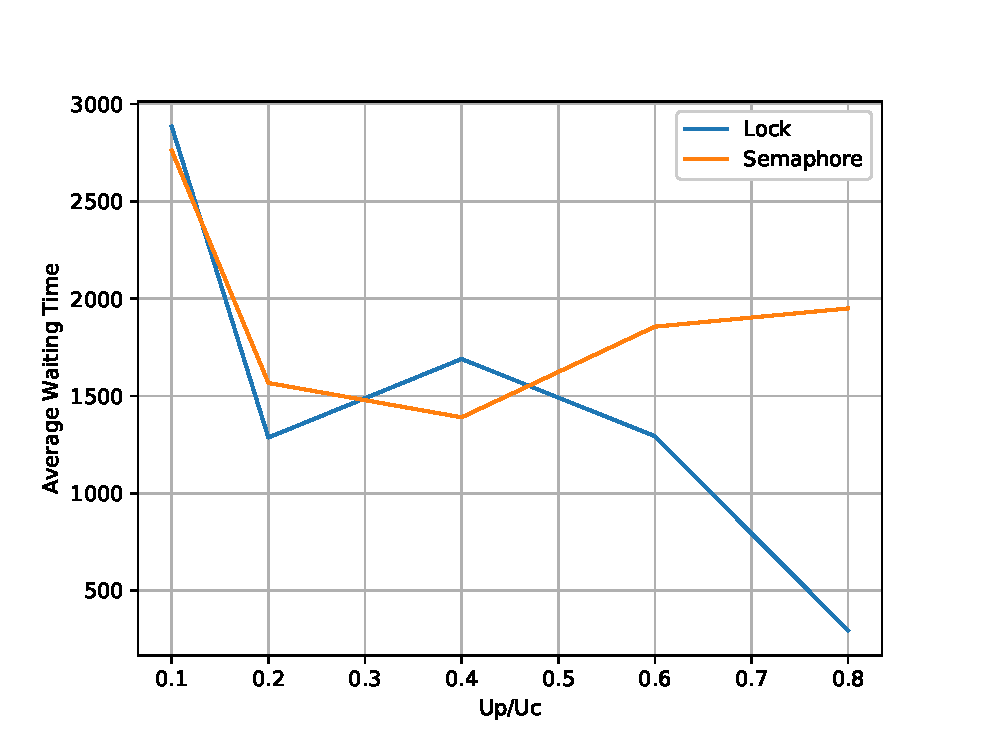
\includegraphics[scale=0.7]{producerd.eps}
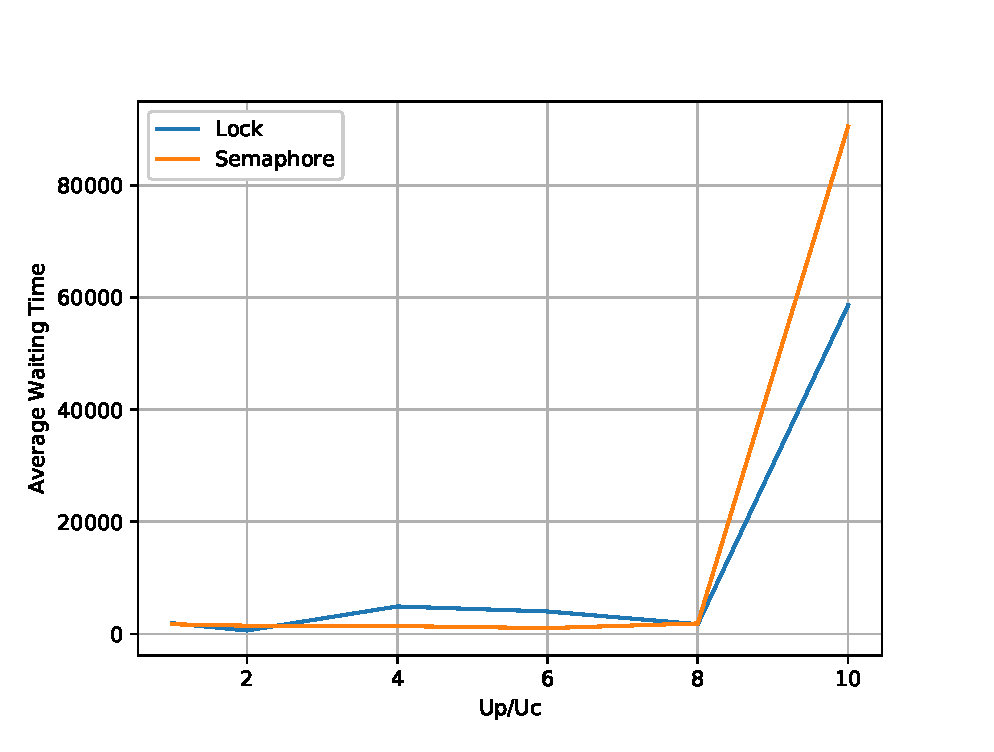
\includegraphics[scale=0.7]{producer.eps}
\end{center}
\newpage
\begin{center}
\begin{large}
\textbf{Consumer Waiting Times vs Ratio of Mean Waiting Times}\\
\end{large}
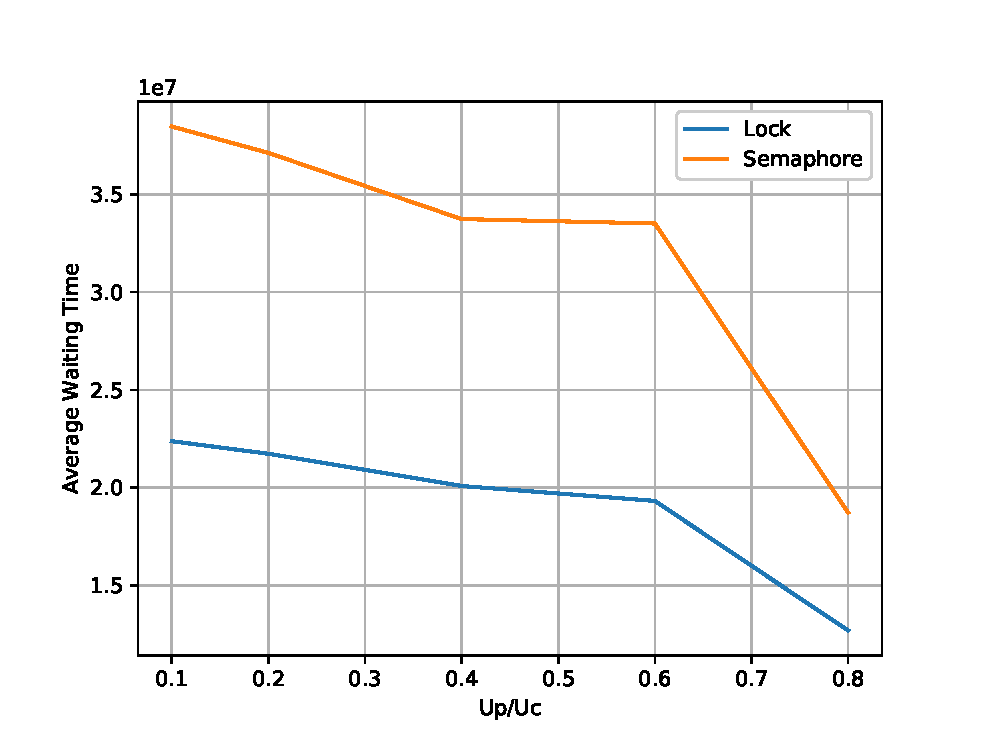
\includegraphics[scale=0.7]{consumerd.eps}
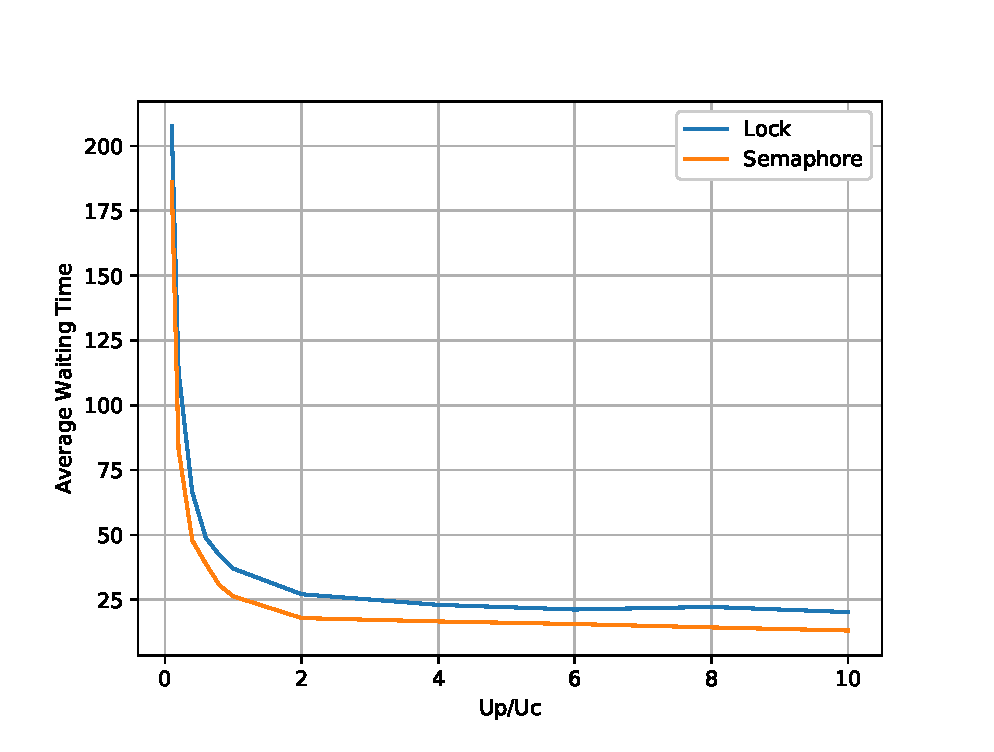
\includegraphics[scale=0.7]{consumer.eps}
\end{center}
\newpage
\section{Explaination of Results}
\begin{enumerate}
\item From the graphs it is quite obvioius that locks perform better than semaphores.
\item This could be due to the fact that sleeping and waking a thread up is a very expensive task.
\item  It is better to busy wait in this case.
\item It is visible that for large values the difference is clear between semphores and locks.
\item Busy wait is not suggested when there is only one core available.
\item One can use locks when there are multiple cores available, otherwise eventhough the semaphores perform worse sleeping of threads seems better than busy waiting. 
\end{enumerate}
\end{document}